\appendix
\chapter{Additional Background}
\section{Pure Arbitrage}
\label{appendix:add-background-pure-arb}
As mentioned in Chapter \ref{sec:pure-arb}, research into this topic is still in its infancy thus which means a very thin slice of exploration on the subject matter. The majority of the research has been into the arbitrage on centralised exchanges~\cite{MakarovIgor2020Taai, crepelliere_arbitrage_2022, PAUNACristian2018ATSf}. Cristian Pauna investigates and implements an arbitrage strategy in~\cite{PAUNACristian2018ATSf}. The paper details the technical details of arbitrage trading from the data and the system architecture used. Pauna finds complications such as requesting data from multiple exchanges, converting the data such that it is homogeneous and also managing server load. Pauna presents the architecture such that the servers request data from the necessary exchanges, aggregating prices in a relational database which then triggers a server that is used to generate trading signals.
\\[3mm]
\begin{figure}[!htb]
    \centering
    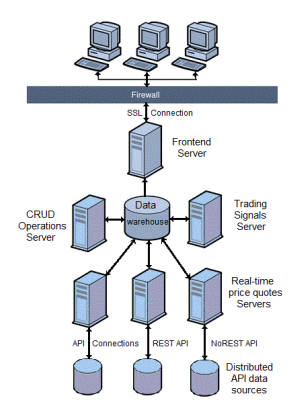
\includegraphics[width=0.28\textwidth]{background/Images/Arbitrage-Architecture.png}
    \caption{Arbitrage system architecture~\cite{PAUNACristian2018ATSf}}
\end{figure}

\noindent Triangular and cyclic arbitrage is one of the most used and purest forms of arbitrage to implement and analyse,~\cite{boonpeam2021arbitrage} explores triangular arbitrage on decentralised exchanges. Algorithm \ref{alg:arb_sys_on_dex} is the algorithm used to find the most profitable arbitrage route on a particular platform, once this is calculated, it is compared with other routes on other platforms. Initially, the system converts the base token into another token and converts it back into the base token, using only one token is used as a middle route, then using the algorithm below, increases the number of middle tokens.
\\[3mm]

\begin{algorithm}
    \caption{Maximum Profit Route Searching (R)}\label{alg:arb_sys_on_dex}
    \textbf{Input}: $T$ (token list), $P$ (price graph), $n$ (current route)
    \begin{algorithmic}
        \For{$i = 1, ..., T$}
        \State $r = get\_profit(n+i)$
        \For{$j = 1,...,P[i]$}
        \State $p = max(r, R(T, P, n_j))$
        \EndFor
        \EndFor
        \State \textbf{return} $p$
    \end{algorithmic}
\end{algorithm}

\noindent On evaluating the performance of the strategy on differing platforms depended on three main features of each exchange:
\begin{enumerate}
    \item Portion size - Depending on how much the ``trader'' invested revenues differed and with the larger portion size, the revenue decreases as the token pair prices are adjusted based on supply/demand.
    \item Transaction fees - Each exchange has its own transaction fee.
    \item Other considerations such as price slippage - Exchanges have different liquidity levels which depend on the usage and liquidity providers that the exchange employs.
\end{enumerate}

\noindent Figure \ref{fig:arb_on_diff_exchanges} displays the revenues obtained by same trading token route, ETH $\rightarrow$ MKR $\rightarrow$ OMG $\rightarrow$ USDT $\rightarrow$ ETH. As we can see upon applying the strategy on multiple exchanges; Uniswap, 1inch, Kyberswap and Bancor, 1 inch was the only exchange that generated a profit whereas the others lose money~\cite{boonpeam2021arbitrage}. 
\\[3mm]
\begin{figure}[!htb]
    \centering
    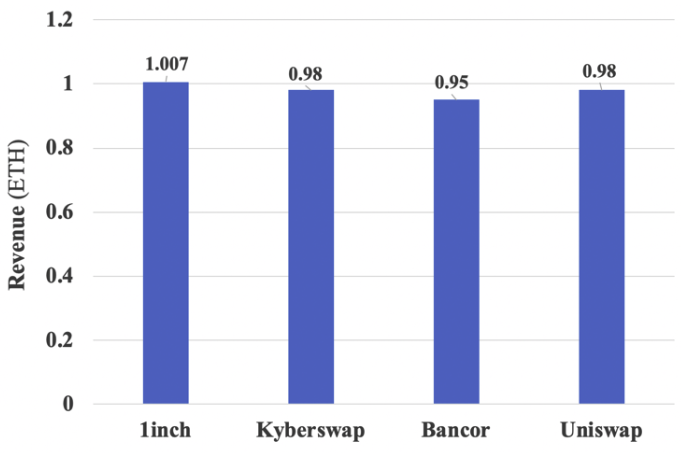
\includegraphics[width=0.6\textwidth]{background/Images/revenue_oncyclic_arb.png}
    \caption{Trading profits same token routes within different exchanges~\cite{boonpeam2021arbitrage} \label{fig:arb_on_diff_exchanges}}
\end{figure}

\noindent Another paper that implemented and evaluated a cyclic arbitrage opportunity is~\cite{wang_cyclic_2022}. The research consists of proposing a theoretical arbitrage model and further evaluation of real transactional data. The arbitrage model used is simple to understand, as it searches for a cyclic transaction between $n$ tokens, $A_1, A_2, ..., A_n$ is a sequence of $n$ trades:
\begin{center}
    \begin{minipage}[c]{0.4\linewidth}
        \begin{itemize}
            \item[\textit{Trade 1:}] Exchange $\delta_1$ of $A_1$ to $\delta_2$ of $A_2$
            \item[\textit{Trade 2:}] Exchange $\delta_2$ of $A_2$ to $\delta_3$ of $A_3$
            \item[] $\dotsc$
            \item[\textit{Trade n:}] Exchange $\delta_n$ of $A_n$ to $\delta_1'$ of $A_1$
        \end{itemize}
    \end{minipage}
\end{center}

\noindent It is important to note that $\delta_i = \delta_{i+1}$, i.e. the output of trade is equivalent to the input of the next. The revenues within a cycle are defined as $\delta_{i+1} - \delta_i$, and the overall profit is $\delta_{1}' - \delta_1$. This is not as simple as the revenues depend on how liquid the exchange is, thus the liquidity pools of each possible trading pair are hugely important. Therefore, the paper proposes a theorem, below:

\begin{theorem}
    For a given cycle $A_1 \rightarrow A_2 \rightarrow \cdots \rightarrow A_n \rightarrow A_1$ with $n$ tokens, there exists an arbitrage opportunity for the cyclic transaction if the product of exchange rates $\frac{a_{2,1}a_{3,2}\cdots a_{1,n}}{a_{1,2}a_{2,3}\cdots a_{n, 1}} > \frac{1}{r_1^n r_2^n}$ where $a_{i,j}$ denotes the liquidity of token $A_i$ in the liquidity pool with token $A_j$.~\cite{wang_cyclic_2022}
\end{theorem}

\noindent In addition to the theorem, to obtain an optimal strategy we need to compute the optimal trading volume of a cycle, $A_1 \rightarrow A_2 \rightarrow \cdots \rightarrow A_n \rightarrow A_1$. The paper proposes the optimal trading volume to be $\delta^{op}_a = \frac{\sqrt{r_1 r_2 a' a} - a}{r_1}$ where $a = \frac{a_{1,n}'a_{n,1}}{a_{n,1}+r_1 r_2 a_{n,1}'}$ and $a' = \frac{r_1 r_2 a_{1,n}'a_{n,1}}{a_{n,1}+r_1 r_2 a_{n,1}'}$. Thus to calculate such arbitrage opportunities knowing the liquidity of tokens in other tokens' liquidity pools, algorithm \ref{alg:liquidity_alg} infers the direction and volumes to trade to get the optimal revenue.

\begin{algorithm}
    \caption{Computing the equivalent liquidity of the cycle}\label{alg:liquidity_alg}
    \begin{algorithmic}
        \State $a_{1, n}' \leftarrow a_{1,2}$
        \State $a_{n, 1}' \leftarrow a_{2,1}$
        \For{$i$ from $2$ to $n-1$}
        \State $a_{1, n}' \leftarrow \frac{a_{1,n}'a_{i,i+1}}{a_{i,i+1}+r_1 r_2 a_{n,1}'}$
        \State $a_{n, 1}' \leftarrow \frac{r_1 r_2 a_{1,n}'a_{i+1, i}}{a_{i,i+1}+r_1 r_2 a_{n,1}'}$
        \EndFor
    \end{algorithmic}
\end{algorithm}

\noindent After analyzing Ethereum block data and applying this strategy to identify the number of arbitrage opportunities, it was found that between May 4, 2020, and April 15, 2021, there were numerous exploitable and profitable arbitrage opportunities. These opportunities grew consistently to reach 1,750 in 11 months, as depicted in Figure \ref{fig:exploitable_ops}. Only cycles with length 3 were experimented with and only cycles including ETH as 80\% of the liquidity pools on Uniswap include ETH and another cryptocurrency~\cite{heimbach2021behavior}. Furthermore, it is found that 287,241 of the 292,606 arbitrages executed started with ETH, and 85\% of the arbitrages used a cycle of length 3. The total revenue of the cyclic arbitrage was 34,429 ETH. However, gas fees account for 24.6\% of the total revenue leaving an approximate 25,971 ETH profit.
\\[3mm]
\begin{figure}[!htb]
    \centering
    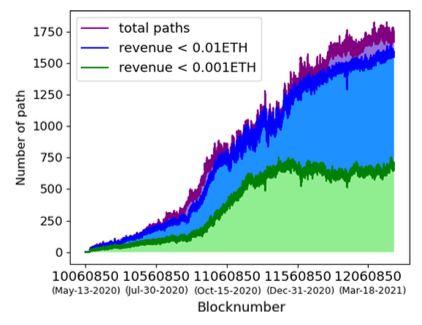
\includegraphics[width=0.6\textwidth]{background/Images/exploitable_ops.png}
    \caption{Number of exploitable opportunities in Uniswap V2 over time. The purple line represents the number of cycles that provide revenue higher than 0.0001 ETH. The green represents the number of cycles whose revenue is under 0.001 ETH. The blue line represents the number of cycles whose revenue is under 0.01 ETH.~\cite{wang_cyclic_2022} \label{fig:exploitable_ops}}
\end{figure}

\noindent The paper then delves into the implementation of the smart contract, and explores how both \textit{sequential} and \textit{atomic} implementations would affect the revenue and execution of the contracts. It was found that 52.3\% of the arbitrages that were executed sequentially generated a loss, likely due to the fact that, when one submits $n$ orders, the $n$ blockchain transactions are executed sequentially, meaning some external transactions can be inserted between these transactions. Thus using atomic transactions avoids this issue of external transactions does not affect the market price that may affect the outcome of the arbitrage.
\\[3mm]
Furthermore, the authors of the paper also investigated the performance differences between using private smart contracts and public contracts. Deploying a smart contract that calls Uniswap functions, i.e. a private smart contract, is intuitively better and achieves a higher success rate of a lower bound of 52\% and a higher bound of 90\% in comparison to calling a public Uniswap smart contract which has a success rate of 27.3\%. Overall the paper provides an insightful look into cyclic arbitrage in DEXes and highlights important decisions made such as liquidity calculations and smart contracts while comparing the performance of different options available.

\section{Optimal Portfolio Design for Mean Reversion}
\label{appendix:add-background-opt-portfolio-des-mean-revers}
There has been further research into optimizing mean reversion, one of which was to use the successive convex approximation method on the mean reverting portfolio design ~\cite{ZipingZhao2019OMPW}. The paper initially proposes the mean reversion portfolio:
\begin{itemize}
    \itemsep0em
    \item For each asset, the price at time $t$ is denoted as $p_t$ and its correspondeing log-price $y_t \triangleq log(p_t)$, its vector form of $M$ assets $\mathbf{y}_t \triangleq \big[ y_{1,t}, \dots ,y_{M,t} \big]^T$.
    \item The log-price spread is given by $y_t \triangleq \mathbf{\beta}^T\mathbf{y}_t$, where $\mathbf{\beta} \triangleq \big[ \beta_1, \dots ,\beta_M \big]^T$ denotes the hedge ratios.
    \item The cointegration space with $N$ relations is defined by $\mathbf{B} \triangleq \big[ \beta_1, \dots ,\beta_N \big]$, thus the $N$ spreads are $s_t \triangleq \mathbf{B}^T\mathbf{y}_t$.
    \item For these $N$ spreads, the portfolio weight matrix is denoted as $\mathbf{w} \triangleq \big[ w_1, \dots ,w_N \big]^T$.
    \item The auto-covariance matrix for the spreads $s_t$ is defined as \\ ${M_i \triangleq Cov(s_t, s_{t+i}) = \mathop{\mathbb{E}} \big[ \big( s_t - \mathop{\mathbb{E}} \big[ s_t \big]\big) \big( s_{t+i} - \mathop{\mathbb{E}} \big[ s_{t+i} \big]\big)^T \big]}$
\end{itemize}

\noindent Now that we have defined everything required, we can now formalize the problem. The general problem of mean reversion portfolio design problem is formalized by:
\begin{equation*}
    \begin{aligned}
         & \underset{\mathbf{w}}{\text{minimize}}
         &                                        & F(\mathbf{w}) \triangleq U(\mathbf{w}) + \mu V(\mathbf{w}) + \gamma S(\mathbf{w})                                                                       \\
         & \text{subject to}
         &                                        & \mathbf{w} \in \biggl\{ \mathbf{w} \mid \big\| \mathbf{B} \mathbf{w}\big\|_0 \leq L \biggr\}, \qquad \text{where $L$ is the total leveraged investment}
    \end{aligned}
\end{equation*}

\begin{itemize}
    \item $\mu$ defines the trade-off between the mean reversion measure and the variance preference.
    \item $\gamma$ defines the regularization parameter of how sparse we would like the cointegration space to be.
\end{itemize}

\noindent Where the Mean Reversion term: $$U(\mathbf{w}) \triangleq \xi \frac{\mathbf{w}^T \mathbf{H}\mathbf{w}}{\mathbf{w}^T \mathbf{M}_0\mathbf{w}} + \zeta \biggl( \frac{\mathbf{w}^T \mathbf{M}_1\mathbf{w}}{\mathbf{w}^T \mathbf{M}_0\mathbf{w}} \biggr) ^2 + \eta \sum_{i=2}^{p} \biggl( \frac{\mathbf{w}^T \mathbf{M}_i\mathbf{w}}{\mathbf{w}^T \mathbf{M}_0\mathbf{w}}\biggr)^2$$ And the variance term: $$V(\mathbf{w}) \triangleq \begin{cases}
        1/\mathbf{w}^T \mathbf{M}_0\mathbf{w}        & \text{VarInv(\textbf{w})} \\
        1/\sqrt{\mathbf{w}^T \mathbf{M}_0\mathbf{w}} & \text{StdInv(\textbf{w})} \\
        -\mathbf{w}^T \mathbf{M}_0\mathbf{w}         & \text{VarNeg(\textbf{w})} \\
        -\sqrt{\mathbf{w}^T \mathbf{M}_0\mathbf{w}}  & \text{StdNeg(\textbf{w})}
    \end{cases}$$
The variance term can be represented in any of the four forms.
\\[3mm]
And the asset selection term: $$S(\mathbf{w}) \triangleq \big\| \mathbf{B} \mathbf{w}\big\|_0 = \sum_{m=1}^{M} sgn(\mid \bigl[ \mathbf{B} \mathbf{w} \bigr]_m \mid)$$ This asset selection criterion is not necessary however as trading incurs a cost, selecting all of the assets is costly, thus selecting a subset of assets to trade is more profitable. To formalize this goal, we would like to minimize the cointegration space thus we use the $\ell_0$ norm.
\\[3mm]
The paper then goes on to solve the optimization problem using the successive convex approximation (SCA) method~\cite{scaOptimization}. The SCA method takes an optimization problem in the form of:
\begin{equation*}
    \begin{aligned}
         & \underset{\mathbf{x}}{\text{minimize}}
         &                                        & f(\mathbf{x})              \\
         & \text{subject to}
         &                                        & \mathbf{x} \in \mathcal{X}
    \end{aligned}
\end{equation*}
\noindent Where $\mathcal{X} \subseteq \mathbb{R}^N$ is convex and $f(\mathbf{x})$ is non-convex. The SCA method involves starting at an initial point $\mathbf{x}^{(0)}$ and solving a series of subproblems of surrogate funtions $\tilde{f}(\mathbf{x}; \mathbf{x}^{(k)})$ over the set $\mathcal{X}$. The sequence $\bigl\{ \mathbf{x}^{(k)} \bigr\}$ is generated by: $$\begin{cases}
        \hat{\mathbf{x}}^{(k+1)} = arg \underset{\mathbf{x} \in \mathcal{X}}{min} \tilde{f}(\mathbf{x}; \mathbf{x}^{(k)}) \\
        \mathbf{x}^{(k+1)} = \mathbf{x}^{(k)} + \gamma^{(k)}(\hat{\mathbf{x}}^{(k+1)} - \mathbf{x}^{(k)})
    \end{cases}$$
The first step is to generate a descent direction and then update the variable with a step size of $\gamma^{(k)}$. After applying this method to the MRP problem and further analysis of the paper, the following algorithm is proposed and used to solve the MRP design problem:
\begin{algorithm}
    \caption{SCA-Based Algorithm for The Optimal MRP Design Problem}\label{alg:sca_alg}
    \textbf{Require}: $\mathbf{H}, \mathbf{M}_i, \mu, \gamma, \mathbf{B}, L \text{ and } \tau$
    \begin{algorithmic}[1]
        \State Set $k=0, \gamma^{(0)}$ and $\mathbf{w}^{(0)}$
        \Repeat
        \State Compute $\mathbf{A}^{(k)}$ and $\mathbf{b}^{(k)}$
        \State $\hat{\mathbf{w}}^{(k+1)} = arg \underset{\mathbf{w} \in \mathcal{W}}{min} \mathbf{w}^{T}\mathbf{A}^{(k)}\mathbf{w} + \mathbf{b}^{(k)T}\mathbf{w}$
        \State $\mathbf{w}^{(k+1)} = \mathbf{w}^{(k)} + \gamma^{(k)}(\hat{\mathbf{w}}^{(k+1)} - \mathbf{w}^{(k)})$
        \State $k \leftarrow k+1$
        \Until convergence
    \end{algorithmic}
\end{algorithm}

\noindent However, 4 line is a convex problem and has no closed-form solution thus to solve this subproblem using the ADMM method, this is done by introducing an auxiliary variable $\mathbf{z = Bw}$.
\begin{equation*}
    \begin{aligned}
         & \underset{\mathbf{x, z}}{\text{minimize}}
         &                                           & \mathbf{w}^{T}\mathbf{A}\mathbf{w} + \mathbf{b}^{T}\mathbf{w} \\
         & \text{subject to}
         &                                           & \big\| \mathbf{z} \big\|_1 \leq B, \mathbf{Bw - z=0}
    \end{aligned}
\end{equation*}
\noindent This is then summarized into Algorithm \ref{alg:admm_alg}:
\begin{algorithm}
    \caption{An ADMM-Based Algorithm for Problem on line 4 in Algorithm \ref{alg:sca_alg}}\label{alg:admm_alg}
    \textbf{Require}: $\mathbf{A}, \mathbf{b}, \mathbf{B}, B, \rho$
    \begin{algorithmic}[1]
        \State Set $\mathbf{w}^{(0)}, \mathbf{z}^{(0)}, \mathbf{u}^{(0)}$ and $k=0$
        \Repeat
        \State $\mathbf{w}^{(k+1)} = -(2\mathbf{A} + \rho \mathbf{B}^T\mathbf{B})^{-1}(\mathbf{b} + \rho \mathbf{B}^T(\mathbf{u}^{(k)} - \mathbf{z}^{(k)}))$
        \State $\mathbf{h}^{(k)} = \mathbf{Bw}^{(k+1)} + \mathbf{u}^{(k)}$
        \State $\mathbf{z}^{(k+1)} = \Pi_{\mathcal{C}}(\mathbf{h}^{(k)})$
        \State $\mathbf{u}^{(k+1)} = \mathbf{u}^{(k)} + \mathbf{Bw}^{(k+1)} - \mathbf{z}^{(k+1)}$
        \State $k \leftarrow k+1$
        \Until convergence
    \end{algorithmic}
\end{algorithm}

\noindent After all of this analysis, the authors of the paper, \cite{8450775, ZipingZhao2019OMPW}, ran simulations on real data comparing underlying spread. It found that it resulted in consistent profits as shown in Figure \ref{fig:ROIsMRP}.
\\[3mm]
\begin{figure}[htb!]
    \centering
    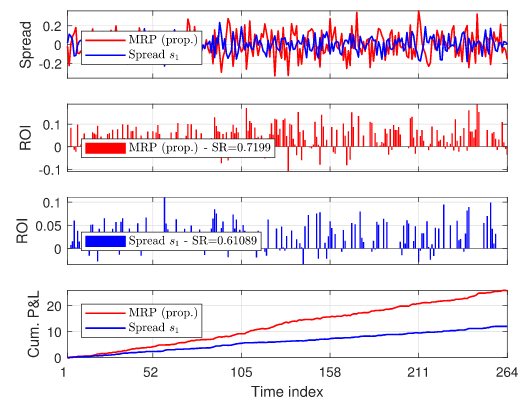
\includegraphics[width=0.4\textwidth]{background/Images/rois1.png}
    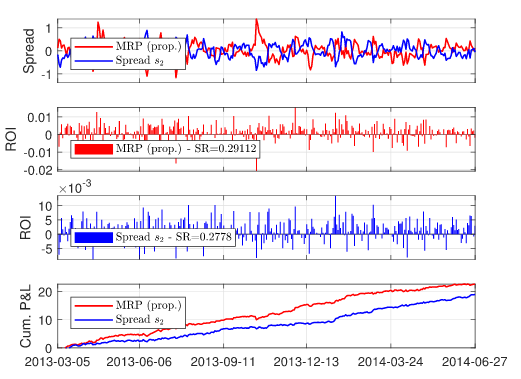
\includegraphics[width=0.43\textwidth]{background/Images/rois2.png}
    \caption{A mean-reversion trading based on real data~\cite{ZipingZhao2019OMPW}}
    \label{fig:ROIsMRP}
\end{figure}

\noindent Overall, this research successfully formulizes, solves the optimization problem mathematically, and goes further to implement the algorithms to solve the problem programmatically. In addition, the author compares the implementation with other benchmark algorithms, showing that it results in a greater P\&L and Sharpe ratio.